\documentclass[12pt,letterpaper]{report}

\usepackage[margin=0.25in]{geometry}
\geometry{
  top=0.8in,            
  inner=1.0in,
  outer=1.0in,
  bottom=0.9in,
  headheight=4ex,       
  headsep=6.5ex,         
}

\setcounter{secnumdepth}{3}
\setcounter{tocdepth}{3}

\usepackage[utf8]{inputenc}
\usepackage[utf8]{vietnam}
\usepackage[english]{babel}
\usepackage{float}
\usepackage{xcolor}
\usepackage{verbatim}
\usepackage{charter}
\usepackage{amsmath}
\usepackage{appendix}
\usepackage{ragged2e}
\usepackage{array}
\usepackage{etoolbox}
\usepackage{fancyhdr}
\usepackage{booktabs}
\usepackage{arydshln}
\usepackage[format=hang,labelfont=bf]{caption}
\usepackage{subcaption}
\usepackage{enumitem}
\usepackage{amssymb}
\usepackage{graphicx}
\usepackage{mathtools}
\usepackage{multirow}
\usepackage{pdfpages}
\usepackage{subfiles}
\usepackage[compact]{titlesec}
\usepackage{stfloats}
\usepackage[style=ieee]{biblatex}
\usepackage{subfiles}
\usepackage[acronym]{glossaries}
\usepackage{gensymb}
\usepackage{algorithm}
\usepackage{algpseudocode}
\usepackage{nameref}

% UML diagram
\usepackage{plantuml}

\usepackage{hyperref}
\hypersetup{
    colorlinks=true,
    linkcolor=blue,
    filecolor=magenta,      
    urlcolor=cyan,
    pdftitle={Overleaf Example},
    pdfpagemode=FullScreen,
    }

\addbibresource{datasheet_ref.bib}
\addbibresource{temp_ref.bib}

\title{PowerMeterOutline}
\author{Quan Dao Nguyen Anh}
\date{July 2023}

\begin{document}

\maketitle

\tableofcontents
\listoffigures
\listoftables

\chapter{Introduction} 

\chapter{Circuit design}

\begin{figure}[!h]
  \centerline{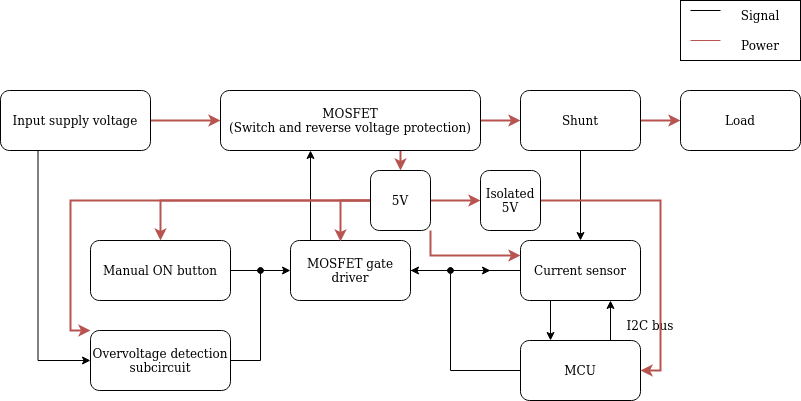
\includegraphics[width=\linewidth]{media/circuit_diagram.drawio.png}}
  \caption{Subcircuits connection: power and signal.}
  \label{fig:Circuit flowchart}
\end{figure}

\justify
In this chapter, the following aspects of designing this project's circuit are discussed:
\begin{enumerate}
  \item MOSFET selection.
  \item MOSFET driver.
  \item Power rail.
  \item Latch and overvoltage detection subcircuit.
  \item Sensor and MCU.
\end{enumerate}

\pagebreak
\subfile{circuit_design/MOSFET_selection.tex}
\pagebreak
\subfile{circuit_design/MOSFET_driver.tex}
\pagebreak
\subfile{circuit_design/power_rail.tex}
\pagebreak
\subfile{circuit_design/latch_circuit.tex}
\pagebreak
\subfile{circuit_design/sensor_mcu.tex}

\chapter{PCB layout}
\justify
In this chapter, the following key design points of the PCB layout are discussed:
\begin{itemize}
  \item Thermal via for TO-263/D2PAK footprint.
  \item Amass XT60PW connector.
\end{itemize}
\pagebreak
\subfile{circuit_design/pcb_layout.tex}

\chapter{Firmware}
\justify
In this chapter, FreeRTOS is first discussed as it is an important component in the firmware of the MCU. Then, the firmware flowchart is discussed. The firmware of the MCU is built by running asynchronous tasks utilizing FreeRTOS with limited shared resources to limit bottlenecking.
\pagebreak
\subfile{firmware/firmware.tex}

\chapter{Application}
\justify
In this chapter, the application is discussed. The application is run on the user/client's PC/laptop. The application is built using Flask, a web application framework written in Python.
\pagebreak
\subfile{application/application.tex}

\chapter{Result}

\printbibliography

\end{document}
